\section{Showcase}
\begin{frame}
    \frametitle{Showcase}
    \framesubtitle{Problem definition and solution}
    To show aspects of our editor we run a modified example proposed by Godiksen et al.
    \pepm. We extend the editor to support addition and want to perform
    step-wise evaluation of the following AST.
    \begin{equation}
        \cursor{\app{\app{\abs{a}{\abs{b}{(a + b)}}}{1}}{(5 + 2)}}
    \end{equation}
    \pause
    We toggle breakpoints along the steps.
    \begin{equation}
        \cursor{\breakpoint{\breakpoint{\app{\app{\abs{a}{\abs{b}{\breakpoint{a + b}}}}{1}}}{\breakpoint{5 + 2}}}}
    \end{equation}
    \pause
    We define a recursive editor expression to evaluate a step.
    \small{
        \begin{align}
             & \rec{x}{                                                                                                                                                                          \\
             & \bicond{\conjunction{\at{\aamLambda{z}}}{\possibly{\aamBreak}}}{\seqcomp{\pre{\child{1}}{\nil}}{\seqcomp{\call{x}}{\pre{\parent}{\nil}}}}{                                        \\
             & \bicond{\conjunction{\at{\aamApp}}{\conjunction{\neg{\necessarily{\aamBreak}}}{\possibly{\aamBreak}}}}{\seqcomp{\pre{\child{1}}{\nil}}{\seqcomp{\call{x}}{\pre{\parent}{\nil}}}}{ \\
             & \bicond{\conjunction{\at{\aamApp}}{\necessarily{\aamBreak}}}{\seqcomp{\pre{\child{2}}{\nil}}{\seqcomp{\call{x}}{\pre{\parent}{\nil}}}}{                                           \\
             & \bicond{\at{\aamBreak}}{\pre{\eval}{\pre{\sub{\aamBreak}}}{\nil}}{\nil}
                        }
                    }
                }
            }
        \end{align}
    }
\end{frame}

\begin{frame}
    \frametitle{Showcase}
    \framesubtitle{Running the solution in our editor - initial}
    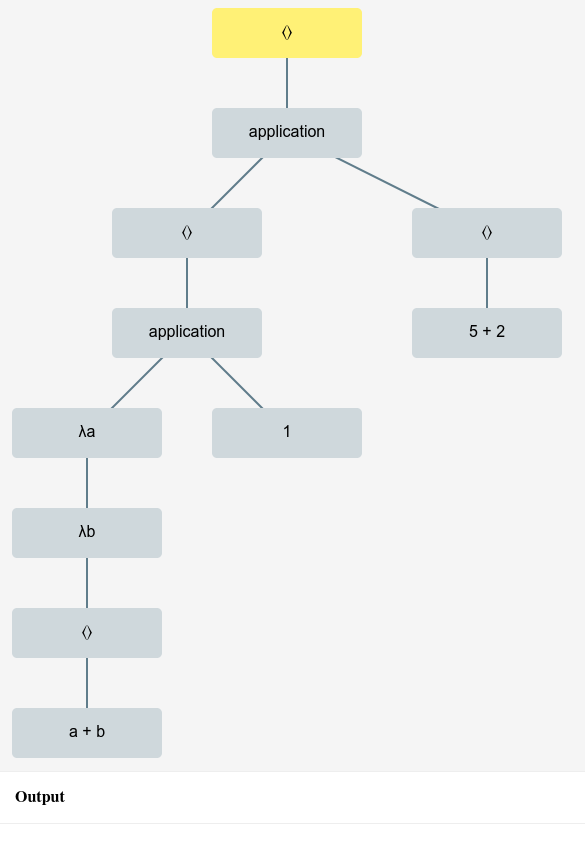
\includegraphics[width=\textwidth, height=8cm]{i0.png}
\end{frame}

\begin{frame}
    \frametitle{Showcase}
    \framesubtitle{Running the solution in our editor - iteration 1}
    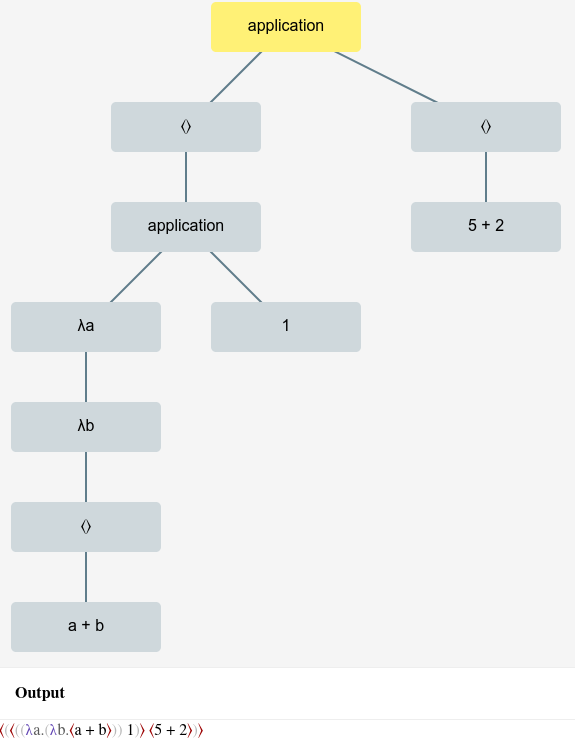
\includegraphics[width=\textwidth, height=8cm]{i1.png}
\end{frame}

\begin{frame}
    \frametitle{Showcase}
    \framesubtitle{Running the solution in our editor - iteration 2}
    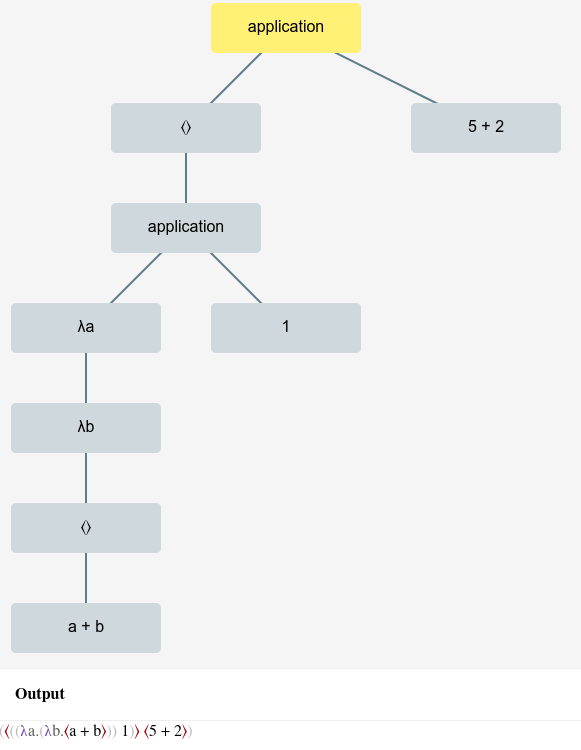
\includegraphics[width=\textwidth, height=8cm]{i2.png}
\end{frame}

\begin{frame}
    \frametitle{Showcase}
    \framesubtitle{Running the solution in our editor - iteration 3}
    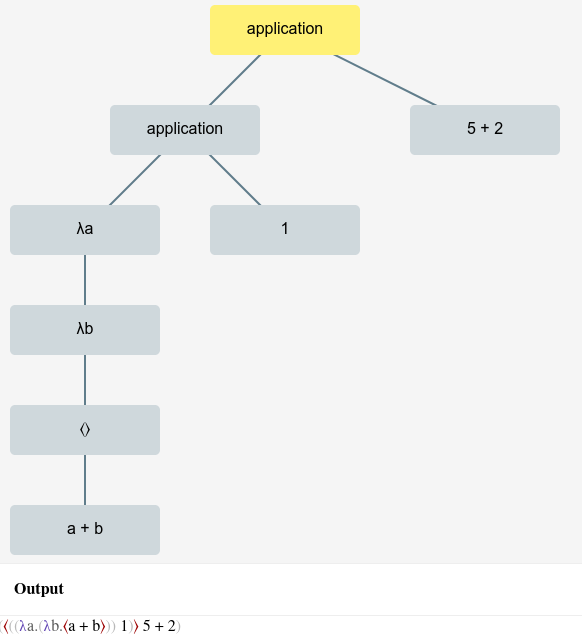
\includegraphics[width=\textwidth, height=8cm]{i3.png}
\end{frame}

\begin{frame}
    \frametitle{Showcase}
    \framesubtitle{Running the solution in our editor - iteration 4}
    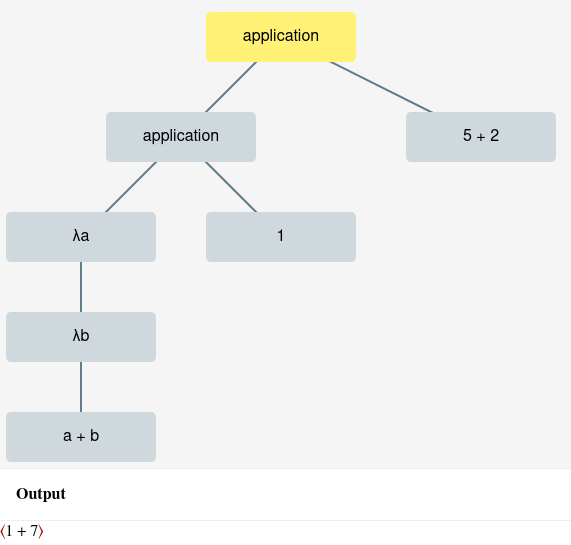
\includegraphics[width=\textwidth, height=8cm]{i4.png}
\end{frame}
